\documentclass[varwidth=18.6cm, border=2pt]{standalone}
\usepackage{tikz}
\usepackage{amsmath,amssymb}
\usetikzlibrary{arrows.meta,shapes.misc}
\definecolor{vertfill}{HTML}{F5A623}
\definecolor{lbltext}{HTML}{1F3B73}
\definecolor{arcgray}{HTML}{C6C6C6}
\definecolor{hired}{HTML}{B03030}
\definecolor{basefill}{HTML}{ECECEC}
\definecolor{okgreen}{HTML}{2E6B34}
\tikzset{
  vtx/.style={circle, draw=lbltext, fill=vertfill, inner sep=0pt, minimum size=5.4mm, font=\scriptsize\bfseries, text=lbltext},
  arc/.style={-{Stealth[length=1.4mm]}, draw=arcgray, line width=0.4pt},
  barc/.style={-{Stealth[length=2.0mm]}, draw=black, line width=1.3pt},
  darc/.style={-{Stealth[length=1.8mm]}, draw=hired, line width=0.9pt, dash pattern=on 1.7pt off 1.3pt},
  cell/.style={draw=lbltext!45, line width=0.3pt},
  cellnew/.style={draw=hired, line width=1.0pt},
  lbl/.style={font=\small, text=lbltext, inner sep=0pt},
  vname/.style={font=\small, text=lbltext, anchor=east, inner sep=0pt},
  slottick/.style={draw=lbltext!55, line width=0.3pt},
  slotnum/.style={font=\tiny, text=lbltext!75, inner sep=0pt},
  tup/.style={font=\small, inner sep=0pt, anchor=west},
  tupdead/.style={font=\small, text=black!35, inner sep=1pt, anchor=west, strike out, draw=black!35},
  key/.style={font=\small, inner sep=0pt, align=left},
  keyhi/.style={font=\small, text=hired, inner sep=0pt},
  keygood/.style={font=\small, text=okgreen, inner sep=0pt},
  keydead/.style={font=\small, text=black!40, inner sep=0pt},
  keydim/.style={font=\small, text=black!55, inner sep=0pt},
  hdr/.style={font=\small\itshape, text=black!65, inner sep=0pt},
  ttl/.style={font=\bfseries, text=lbltext, anchor=west, inner sep=0pt},
  bad/.style={font=\small, text=hired, inner sep=0pt},
  good/.style={font=\small, text=okgreen, inner sep=0pt},
  lift/.style={-{Stealth[length=1.3mm]}, draw=black!50, line width=0.4pt},
  keybox/.style={key, draw=hired, line width=0.7pt, rounded corners=1.5pt, inner xsep=2pt, inner ysep=1.2pt},
}
\newsavebox{\pnlA}\newsavebox{\pnlB}\newsavebox{\pnlC}
\newsavebox{\pnlD}\newsavebox{\pnlE}\newsavebox{\pnlF}
\newlength{\pnlone}\newlength{\pnltwo}\newlength{\pnlthree}
\newlength{\pnlgap}\newlength{\pnlcanvas}
\setlength{\pnlcanvas}{18.6cm}
\newcommand{\pnlcol}[3]{\setlength{#1}{\wd#2}%
  \ifdim\wd#3>#1\relax\setlength{#1}{\wd#3}\fi}
\begin{document}
\sbox{\pnlA}{%
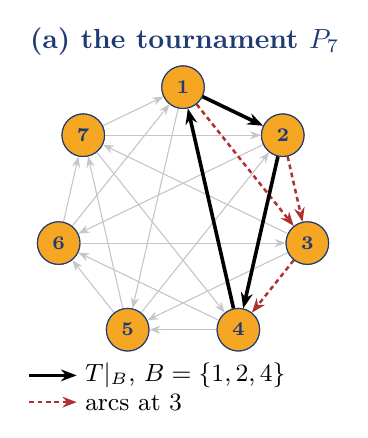
\begin{tikzpicture}[x=1cm,y=1cm,baseline=0cm]
  \node[ttl] at (-1.950,0.000) {(a) the tournament $P_{7}$};
  \node[vtx] (v0) at (0.000,-0.580) {1};
  \node[vtx] (v1) at (1.267,-1.190) {2};
  \node[vtx] (v2) at (1.579,-2.560) {3};
  \node[vtx] (v3) at (0.703,-3.660) {4};
  \node[vtx] (v4) at (-0.703,-3.660) {5};
  \node[vtx] (v5) at (-1.579,-2.560) {6};
  \node[vtx] (v6) at (-1.267,-1.190) {7};
  \draw[arc] (v0) -- (v4);
  \draw[arc] (v1) -- (v5);
  \draw[arc] (v2) -- (v4);
  \draw[arc] (v2) -- (v6);
  \draw[arc] (v3) -- (v4);
  \draw[arc] (v3) -- (v5);
  \draw[arc] (v4) -- (v1);
  \draw[arc] (v4) -- (v5);
  \draw[arc] (v4) -- (v6);
  \draw[arc] (v5) -- (v0);
  \draw[arc] (v5) -- (v2);
  \draw[arc] (v5) -- (v6);
  \draw[arc] (v6) -- (v0);
  \draw[arc] (v6) -- (v1);
  \draw[arc] (v6) -- (v3);
  \draw[darc] (v2) -- (v3);
  \draw[darc] (v0) -- (v2);
  \draw[darc] (v1) -- (v2);
  \draw[barc] (v0) -- (v1);
  \draw[barc] (v1) -- (v3);
  \draw[barc] (v3) -- (v0);
  \node[vtx] at (v0) {1};
  \node[vtx] at (v1) {2};
  \node[vtx] at (v2) {3};
  \node[vtx] at (v3) {4};
  \node[vtx] at (v4) {5};
  \node[vtx] at (v5) {6};
  \node[vtx] at (v6) {7};
  \draw[barc] (-1.95,-4.240) -- ++(0.60,0);
  \node[key, anchor=west] at (-1.25,-4.240) {$T|_B$, $B=\{1,2,4\}$};
  \draw[darc] (-1.95,-4.580) -- ++(0.60,0);
  \node[key, anchor=west] at (-1.25,-4.580) {arcs at $3$};
\end{tikzpicture}%
}%
\sbox{\pnlB}{%
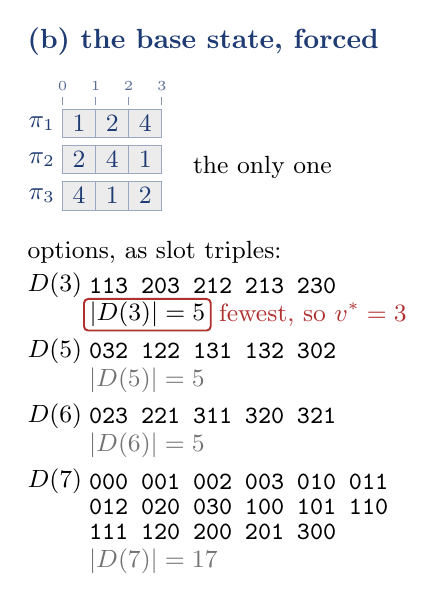
\begin{tikzpicture}[x=1cm,y=1cm,baseline=0cm]
  \node[ttl] at (0.000,0.000) {(b) the base state, forced};
  \draw[slottick] (0.450,-0.810) -- ++(0,0.11);
  \node[slotnum] at (0.450,-0.570) {0};
  \draw[slottick] (0.870,-0.810) -- ++(0,0.11);
  \node[slotnum] at (0.870,-0.570) {1};
  \draw[slottick] (1.290,-0.810) -- ++(0,0.11);
  \node[slotnum] at (1.290,-0.570) {2};
  \draw[slottick] (1.710,-0.810) -- ++(0,0.11);
  \node[slotnum] at (1.710,-0.570) {3};
  \node[vname] at (0.360,-1.040) {$\pi_{1}$};
  \draw[cell, fill=basefill] (0.450,-1.220) rectangle ++(0.420,0.360);
  \node[lbl] at (0.660,-1.040) {1};
  \draw[cell, fill=basefill] (0.870,-1.220) rectangle ++(0.420,0.360);
  \node[lbl] at (1.080,-1.040) {2};
  \draw[cell, fill=basefill] (1.290,-1.220) rectangle ++(0.420,0.360);
  \node[lbl] at (1.500,-1.040) {4};
  \node[vname] at (0.360,-1.500) {$\pi_{2}$};
  \draw[cell, fill=basefill] (0.450,-1.680) rectangle ++(0.420,0.360);
  \node[lbl] at (0.660,-1.500) {2};
  \draw[cell, fill=basefill] (0.870,-1.680) rectangle ++(0.420,0.360);
  \node[lbl] at (1.080,-1.500) {4};
  \draw[cell, fill=basefill] (1.290,-1.680) rectangle ++(0.420,0.360);
  \node[lbl] at (1.500,-1.500) {1};
  \node[vname] at (0.360,-1.960) {$\pi_{3}$};
  \draw[cell, fill=basefill] (0.450,-2.140) rectangle ++(0.420,0.360);
  \node[lbl] at (0.660,-1.960) {4};
  \draw[cell, fill=basefill] (0.870,-2.140) rectangle ++(0.420,0.360);
  \node[lbl] at (1.080,-1.960) {1};
  \draw[cell, fill=basefill] (1.290,-2.140) rectangle ++(0.420,0.360);
  \node[lbl] at (1.500,-1.960) {2};
  \node[key, anchor=west] at (2.10,-1.600) {the only one};
  \node[key, anchor=west] at (0,-2.680) {options, as slot triples:};
  \node[key, anchor=west] at (0.000,-3.100) {$D(3)$};
  \node[tup, anchor=west] at (0.780,-3.100) {\texttt{113}};
  \node[tup, anchor=west] at (1.440,-3.100) {\texttt{203}};
  \node[tup, anchor=west] at (2.100,-3.100) {\texttt{212}};
  \node[tup, anchor=west] at (2.760,-3.100) {\texttt{213}};
  \node[tup, anchor=west] at (3.420,-3.100) {\texttt{230}};
  \node[keybox, anchor=west] at (0.710,-3.470) {$|D(3)|=5$};
  \node[keyhi, anchor=west] at (2.430,-3.470) {fewest, so $v^{*}=3$};
  \node[key, anchor=west] at (0.000,-3.930) {$D(5)$};
  \node[tup, anchor=west] at (0.780,-3.930) {\texttt{032}};
  \node[tup, anchor=west] at (1.440,-3.930) {\texttt{122}};
  \node[tup, anchor=west] at (2.100,-3.930) {\texttt{131}};
  \node[tup, anchor=west] at (2.760,-3.930) {\texttt{132}};
  \node[tup, anchor=west] at (3.420,-3.930) {\texttt{302}};
  \node[keydim, anchor=west] at (0.780,-4.300) {$|D(5)|=5$};
  \node[key, anchor=west] at (0.000,-4.760) {$D(6)$};
  \node[tup, anchor=west] at (0.780,-4.760) {\texttt{023}};
  \node[tup, anchor=west] at (1.440,-4.760) {\texttt{221}};
  \node[tup, anchor=west] at (2.100,-4.760) {\texttt{311}};
  \node[tup, anchor=west] at (2.760,-4.760) {\texttt{320}};
  \node[tup, anchor=west] at (3.420,-4.760) {\texttt{321}};
  \node[keydim, anchor=west] at (0.780,-5.130) {$|D(6)|=5$};
  \node[key, anchor=west] at (0.000,-5.590) {$D(7)$};
  \node[tup, anchor=west] at (0.780,-5.590) {\texttt{000}};
  \node[tup, anchor=west] at (1.440,-5.590) {\texttt{001}};
  \node[tup, anchor=west] at (2.100,-5.590) {\texttt{002}};
  \node[tup, anchor=west] at (2.760,-5.590) {\texttt{003}};
  \node[tup, anchor=west] at (3.420,-5.590) {\texttt{010}};
  \node[tup, anchor=west] at (4.080,-5.590) {\texttt{011}};
  \node[tup, anchor=west] at (0.780,-5.910) {\texttt{012}};
  \node[tup, anchor=west] at (1.440,-5.910) {\texttt{020}};
  \node[tup, anchor=west] at (2.100,-5.910) {\texttt{030}};
  \node[tup, anchor=west] at (2.760,-5.910) {\texttt{100}};
  \node[tup, anchor=west] at (3.420,-5.910) {\texttt{101}};
  \node[tup, anchor=west] at (4.080,-5.910) {\texttt{110}};
  \node[tup, anchor=west] at (0.780,-6.230) {\texttt{111}};
  \node[tup, anchor=west] at (1.440,-6.230) {\texttt{120}};
  \node[tup, anchor=west] at (2.100,-6.230) {\texttt{200}};
  \node[tup, anchor=west] at (2.760,-6.230) {\texttt{201}};
  \node[tup, anchor=west] at (3.420,-6.230) {\texttt{300}};
  \node[keydim, anchor=west] at (0.780,-6.600) {$|D(7)|=17$};
\end{tikzpicture}%
}%
\sbox{\pnlC}{%
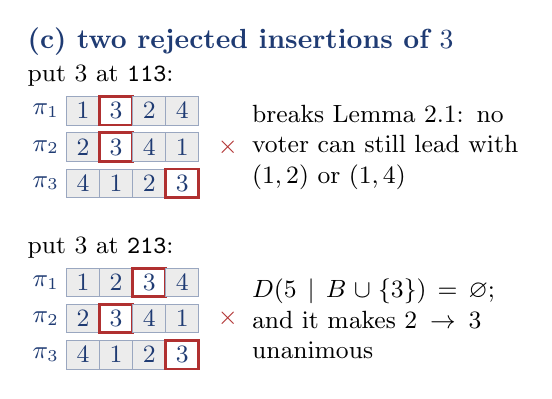
\begin{tikzpicture}[x=1cm,y=1cm,baseline=0cm]
  \node[ttl] at (0.000,0.000) {(c) two rejected insertions of $3$};
  \node[key, anchor=west] at (0,-0.440) {put $3$ at \texttt{113}:};
  \node[vname] at (0.410,-0.880) {$\pi_{1}$};
  \draw[cell, fill=basefill] (0.500,-1.060) rectangle ++(0.420,0.360);
  \node[lbl] at (0.710,-0.880) {1};
  \draw[cellnew, fill=white] (0.920,-1.060) rectangle ++(0.420,0.360);
  \node[lbl] at (1.130,-0.880) {3};
  \draw[cell, fill=basefill] (1.340,-1.060) rectangle ++(0.420,0.360);
  \node[lbl] at (1.550,-0.880) {2};
  \draw[cell, fill=basefill] (1.760,-1.060) rectangle ++(0.420,0.360);
  \node[lbl] at (1.970,-0.880) {4};
  \node[vname] at (0.410,-1.340) {$\pi_{2}$};
  \draw[cell, fill=basefill] (0.500,-1.520) rectangle ++(0.420,0.360);
  \node[lbl] at (0.710,-1.340) {2};
  \draw[cellnew, fill=white] (0.920,-1.520) rectangle ++(0.420,0.360);
  \node[lbl] at (1.130,-1.340) {3};
  \draw[cell, fill=basefill] (1.340,-1.520) rectangle ++(0.420,0.360);
  \node[lbl] at (1.550,-1.340) {4};
  \draw[cell, fill=basefill] (1.760,-1.520) rectangle ++(0.420,0.360);
  \node[lbl] at (1.970,-1.340) {1};
  \node[vname] at (0.410,-1.800) {$\pi_{3}$};
  \draw[cell, fill=basefill] (0.500,-1.980) rectangle ++(0.420,0.360);
  \node[lbl] at (0.710,-1.800) {4};
  \draw[cell, fill=basefill] (0.920,-1.980) rectangle ++(0.420,0.360);
  \node[lbl] at (1.130,-1.800) {1};
  \draw[cell, fill=basefill] (1.340,-1.980) rectangle ++(0.420,0.360);
  \node[lbl] at (1.550,-1.800) {2};
  \draw[cellnew, fill=white] (1.760,-1.980) rectangle ++(0.420,0.360);
  \node[lbl] at (1.970,-1.800) {3};
  \node[bad] at (2.550,-1.340) {$\times$};
  \node[key, anchor=west, text width=3.45cm] at (2.85,-1.340) {breaks Lemma 2.1: no voter can still lead with $(1,2)$ or $(1,4)$};
  \node[key, anchor=west] at (0,-2.620) {put $3$ at \texttt{213}:};
  \node[vname] at (0.410,-3.060) {$\pi_{1}$};
  \draw[cell, fill=basefill] (0.500,-3.240) rectangle ++(0.420,0.360);
  \node[lbl] at (0.710,-3.060) {1};
  \draw[cell, fill=basefill] (0.920,-3.240) rectangle ++(0.420,0.360);
  \node[lbl] at (1.130,-3.060) {2};
  \draw[cellnew, fill=white] (1.340,-3.240) rectangle ++(0.420,0.360);
  \node[lbl] at (1.550,-3.060) {3};
  \draw[cell, fill=basefill] (1.760,-3.240) rectangle ++(0.420,0.360);
  \node[lbl] at (1.970,-3.060) {4};
  \node[vname] at (0.410,-3.520) {$\pi_{2}$};
  \draw[cell, fill=basefill] (0.500,-3.700) rectangle ++(0.420,0.360);
  \node[lbl] at (0.710,-3.520) {2};
  \draw[cellnew, fill=white] (0.920,-3.700) rectangle ++(0.420,0.360);
  \node[lbl] at (1.130,-3.520) {3};
  \draw[cell, fill=basefill] (1.340,-3.700) rectangle ++(0.420,0.360);
  \node[lbl] at (1.550,-3.520) {4};
  \draw[cell, fill=basefill] (1.760,-3.700) rectangle ++(0.420,0.360);
  \node[lbl] at (1.970,-3.520) {1};
  \node[vname] at (0.410,-3.980) {$\pi_{3}$};
  \draw[cell, fill=basefill] (0.500,-4.160) rectangle ++(0.420,0.360);
  \node[lbl] at (0.710,-3.980) {4};
  \draw[cell, fill=basefill] (0.920,-4.160) rectangle ++(0.420,0.360);
  \node[lbl] at (1.130,-3.980) {1};
  \draw[cell, fill=basefill] (1.340,-4.160) rectangle ++(0.420,0.360);
  \node[lbl] at (1.550,-3.980) {2};
  \draw[cellnew, fill=white] (1.760,-4.160) rectangle ++(0.420,0.360);
  \node[lbl] at (1.970,-3.980) {3};
  \node[bad] at (2.550,-3.520) {$\times$};
  \node[key, anchor=west, text width=3.45cm] at (2.85,-3.520) {$D(5\mid B\cup\{3\})=\varnothing$; and it makes $2\to3$ unanimous};
\end{tikzpicture}%
}%
\sbox{\pnlD}{%
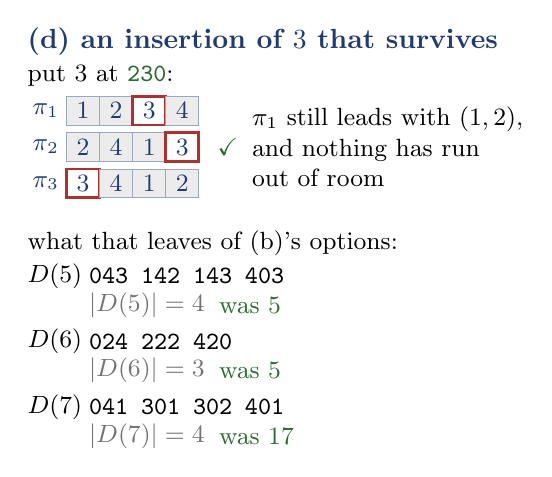
\begin{tikzpicture}[x=1cm,y=1cm,baseline=0cm]
  \node[ttl] at (0.000,0.000) {(d) an insertion of $3$ that survives};
  \node[key, anchor=west] at (0,-0.44) {put $3$ at \textcolor{okgreen}{\texttt{230}}:};
  \node[vname] at (0.410,-0.880) {$\pi_{1}$};
  \draw[cell, fill=basefill] (0.500,-1.060) rectangle ++(0.420,0.360);
  \node[lbl] at (0.710,-0.880) {1};
  \draw[cell, fill=basefill] (0.920,-1.060) rectangle ++(0.420,0.360);
  \node[lbl] at (1.130,-0.880) {2};
  \draw[cellnew, fill=white] (1.340,-1.060) rectangle ++(0.420,0.360);
  \node[lbl] at (1.550,-0.880) {3};
  \draw[cell, fill=basefill] (1.760,-1.060) rectangle ++(0.420,0.360);
  \node[lbl] at (1.970,-0.880) {4};
  \node[vname] at (0.410,-1.340) {$\pi_{2}$};
  \draw[cell, fill=basefill] (0.500,-1.520) rectangle ++(0.420,0.360);
  \node[lbl] at (0.710,-1.340) {2};
  \draw[cell, fill=basefill] (0.920,-1.520) rectangle ++(0.420,0.360);
  \node[lbl] at (1.130,-1.340) {4};
  \draw[cell, fill=basefill] (1.340,-1.520) rectangle ++(0.420,0.360);
  \node[lbl] at (1.550,-1.340) {1};
  \draw[cellnew, fill=white] (1.760,-1.520) rectangle ++(0.420,0.360);
  \node[lbl] at (1.970,-1.340) {3};
  \node[vname] at (0.410,-1.800) {$\pi_{3}$};
  \draw[cellnew, fill=white] (0.500,-1.980) rectangle ++(0.420,0.360);
  \node[lbl] at (0.710,-1.800) {3};
  \draw[cell, fill=basefill] (0.920,-1.980) rectangle ++(0.420,0.360);
  \node[lbl] at (1.130,-1.800) {4};
  \draw[cell, fill=basefill] (1.340,-1.980) rectangle ++(0.420,0.360);
  \node[lbl] at (1.550,-1.800) {1};
  \draw[cell, fill=basefill] (1.760,-1.980) rectangle ++(0.420,0.360);
  \node[lbl] at (1.970,-1.800) {2};
  \node[good] at (2.550,-1.340) {$\checkmark$};
  \node[key, anchor=west, text width=3.45cm] at (2.85,-1.340) {$\pi_1$ still leads with $(1,2)$, and nothing has run out of room};
  \node[key, anchor=west] at (0,-2.560) {what that leaves of (b)'s options:};
  \node[key, anchor=west] at (0.000,-2.980) {$D(5)$};
  \node[tup, anchor=west] at (0.780,-2.980) {\texttt{043}};
  \node[tup, anchor=west] at (1.440,-2.980) {\texttt{142}};
  \node[tup, anchor=west] at (2.100,-2.980) {\texttt{143}};
  \node[tup, anchor=west] at (2.760,-2.980) {\texttt{403}};
  \node[keydim, anchor=west] at (0.780,-3.350) {$|D(5)|=4$};
  \node[keygood, anchor=west] at (2.430,-3.350) {was $5$};
  \node[key, anchor=west] at (0.000,-3.810) {$D(6)$};
  \node[tup, anchor=west] at (0.780,-3.810) {\texttt{024}};
  \node[tup, anchor=west] at (1.440,-3.810) {\texttt{222}};
  \node[tup, anchor=west] at (2.100,-3.810) {\texttt{420}};
  \node[keydim, anchor=west] at (0.780,-4.180) {$|D(6)|=3$};
  \node[keygood, anchor=west] at (2.430,-4.180) {was $5$};
  \node[key, anchor=west] at (0.000,-4.640) {$D(7)$};
  \node[tup, anchor=west] at (0.780,-4.640) {\texttt{041}};
  \node[tup, anchor=west] at (1.440,-4.640) {\texttt{301}};
  \node[tup, anchor=west] at (2.100,-4.640) {\texttt{302}};
  \node[tup, anchor=west] at (2.760,-4.640) {\texttt{401}};
  \node[keydim, anchor=west] at (0.780,-5.010) {$|D(7)|=4$};
  \node[keygood, anchor=west] at (2.430,-5.010) {was $17$};
\end{tikzpicture}%
}%
\sbox{\pnlE}{%
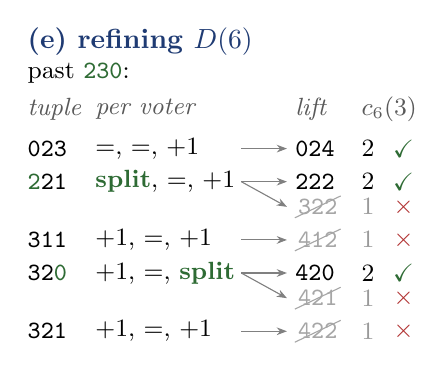
\begin{tikzpicture}[x=1cm,y=1cm,baseline=0cm]
  \node[ttl] at (0.000,0.000) {(e) refining $D(6)$};
  \node[key, anchor=west] at (0,-0.40) {past \textcolor{okgreen}{\texttt{230}}:};
  \node[hdr, anchor=west] at (0,-0.86) {tuple};
  \node[hdr, anchor=west] at (0.86,-0.86) {per voter};
  \node[hdr, anchor=west] at (3.40,-0.86) {lift};
  \node[hdr, anchor=west] at (4.24,-0.86) {$c_{6}(3)$};
  \node[tup, anchor=west] at (0,-1.360) {\texttt{023}};
  \node[key, anchor=west] at (0.86,-1.360) {$=$, $=$, $+1$};
  \draw[lift] (2.72,-1.360) -- (3.30,-1.360);
  \node[tup, anchor=west] at (3.40,-1.360) {\texttt{024}};
  \node[key, anchor=west] at (4.24,-1.360) {$2$};
  \node[good] at (4.780,-1.360) {$\checkmark$};
  \node[tup, anchor=west] at (0,-1.780) {\texttt{\textcolor{okgreen}{2}21}};
  \node[key, anchor=west] at (0.86,-1.780) {\textcolor{okgreen}{\textbf{split}}, $=$, $+1$};
  \draw[lift] (2.72,-1.780) -- (3.30,-1.780);
  \node[tup, anchor=west] at (3.40,-1.780) {\texttt{222}};
  \node[key, anchor=west] at (4.24,-1.780) {$2$};
  \node[good] at (4.780,-1.780) {$\checkmark$};
  \draw[lift] (2.72,-1.780) -- (3.30,-2.100);
  \node[tupdead, anchor=west] at (3.40,-2.100) {\texttt{322}};
  \node[keydead, anchor=west] at (4.24,-2.100) {$1$};
  \node[bad] at (4.780,-2.100) {$\times$};
  \node[tup, anchor=west] at (0,-2.520) {\texttt{311}};
  \node[key, anchor=west] at (0.86,-2.520) {$+1$, $=$, $+1$};
  \draw[lift] (2.72,-2.520) -- (3.30,-2.520);
  \node[tupdead, anchor=west] at (3.40,-2.520) {\texttt{412}};
  \node[keydead, anchor=west] at (4.24,-2.520) {$1$};
  \node[bad] at (4.780,-2.520) {$\times$};
  \node[tup, anchor=west] at (0,-2.940) {\texttt{32\textcolor{okgreen}{0}}};
  \node[key, anchor=west] at (0.86,-2.940) {$+1$, $=$, \textcolor{okgreen}{\textbf{split}}};
  \draw[lift] (2.72,-2.940) -- (3.30,-2.940);
  \node[tup, anchor=west] at (3.40,-2.940) {\texttt{420}};
  \node[key, anchor=west] at (4.24,-2.940) {$2$};
  \node[good] at (4.780,-2.940) {$\checkmark$};
  \draw[lift] (2.72,-2.940) -- (3.30,-3.260);
  \node[tupdead, anchor=west] at (3.40,-3.260) {\texttt{421}};
  \node[keydead, anchor=west] at (4.24,-3.260) {$1$};
  \node[bad] at (4.780,-3.260) {$\times$};
  \node[tup, anchor=west] at (0,-3.680) {\texttt{321}};
  \node[key, anchor=west] at (0.86,-3.680) {$+1$, $=$, $+1$};
  \draw[lift] (2.72,-3.680) -- (3.30,-3.680);
  \node[tupdead, anchor=west] at (3.40,-3.680) {\texttt{422}};
  \node[keydead, anchor=west] at (4.24,-3.680) {$1$};
  \node[bad] at (4.780,-3.680) {$\times$};
\end{tikzpicture}%
}%
\sbox{\pnlF}{%
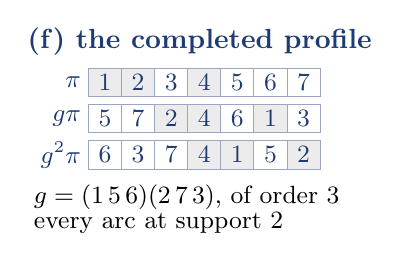
\begin{tikzpicture}[x=1cm,y=1cm,baseline=0cm]
  \node[ttl] at (0.000,0.000) {(f) the completed profile};
  \node[vname] at (0.690,-0.520) {$\pi$};
  \draw[cell, fill=basefill] (0.780,-0.700) rectangle ++(0.420,0.360);
  \node[lbl] at (0.990,-0.520) {1};
  \draw[cell, fill=basefill] (1.200,-0.700) rectangle ++(0.420,0.360);
  \node[lbl] at (1.410,-0.520) {2};
  \draw[cell, fill=white] (1.620,-0.700) rectangle ++(0.420,0.360);
  \node[lbl] at (1.830,-0.520) {3};
  \draw[cell, fill=basefill] (2.040,-0.700) rectangle ++(0.420,0.360);
  \node[lbl] at (2.250,-0.520) {4};
  \draw[cell, fill=white] (2.460,-0.700) rectangle ++(0.420,0.360);
  \node[lbl] at (2.670,-0.520) {5};
  \draw[cell, fill=white] (2.880,-0.700) rectangle ++(0.420,0.360);
  \node[lbl] at (3.090,-0.520) {6};
  \draw[cell, fill=white] (3.300,-0.700) rectangle ++(0.420,0.360);
  \node[lbl] at (3.510,-0.520) {7};
  \node[vname] at (0.690,-0.980) {$g\pi$};
  \draw[cell, fill=white] (0.780,-1.160) rectangle ++(0.420,0.360);
  \node[lbl] at (0.990,-0.980) {5};
  \draw[cell, fill=white] (1.200,-1.160) rectangle ++(0.420,0.360);
  \node[lbl] at (1.410,-0.980) {7};
  \draw[cell, fill=basefill] (1.620,-1.160) rectangle ++(0.420,0.360);
  \node[lbl] at (1.830,-0.980) {2};
  \draw[cell, fill=basefill] (2.040,-1.160) rectangle ++(0.420,0.360);
  \node[lbl] at (2.250,-0.980) {4};
  \draw[cell, fill=white] (2.460,-1.160) rectangle ++(0.420,0.360);
  \node[lbl] at (2.670,-0.980) {6};
  \draw[cell, fill=basefill] (2.880,-1.160) rectangle ++(0.420,0.360);
  \node[lbl] at (3.090,-0.980) {1};
  \draw[cell, fill=white] (3.300,-1.160) rectangle ++(0.420,0.360);
  \node[lbl] at (3.510,-0.980) {3};
  \node[vname] at (0.690,-1.440) {$g^{2}\pi$};
  \draw[cell, fill=white] (0.780,-1.620) rectangle ++(0.420,0.360);
  \node[lbl] at (0.990,-1.440) {6};
  \draw[cell, fill=white] (1.200,-1.620) rectangle ++(0.420,0.360);
  \node[lbl] at (1.410,-1.440) {3};
  \draw[cell, fill=white] (1.620,-1.620) rectangle ++(0.420,0.360);
  \node[lbl] at (1.830,-1.440) {7};
  \draw[cell, fill=basefill] (2.040,-1.620) rectangle ++(0.420,0.360);
  \node[lbl] at (2.250,-1.440) {4};
  \draw[cell, fill=basefill] (2.460,-1.620) rectangle ++(0.420,0.360);
  \node[lbl] at (2.670,-1.440) {1};
  \draw[cell, fill=white] (2.880,-1.620) rectangle ++(0.420,0.360);
  \node[lbl] at (3.090,-1.440) {5};
  \draw[cell, fill=basefill] (3.300,-1.620) rectangle ++(0.420,0.360);
  \node[lbl] at (3.510,-1.440) {2};
  \node[key, anchor=west] at (0.080,-1.980) {$g = (1\,5\,6)(2\,7\,3)$, of order $3$};
  \node[key, anchor=west] at (0.080,-2.300) {every arc at support $2$};
\end{tikzpicture}%
}%
\pnlcol{\pnlone}{\pnlA}{\pnlD}
\pnlcol{\pnltwo}{\pnlB}{\pnlE}
\pnlcol{\pnlthree}{\pnlC}{\pnlF}
\setlength{\pnlgap}{\pnlcanvas}
\addtolength{\pnlgap}{-\pnlone}
\addtolength{\pnlgap}{-\pnltwo}
\addtolength{\pnlgap}{-\pnlthree}
\setlength{\pnlgap}{0.5\pnlgap}
\ifdim\pnlgap<0pt\relax\errmessage{the panels are wider than the \the\pnlcanvas\space canvas: \the\pnlone, \the\pnltwo, \the\pnlthree}\fi
\makebox[\pnlone][l]{\usebox{\pnlA}}\hspace{\pnlgap}%
\makebox[\pnltwo][l]{\usebox{\pnlB}}\hspace{\pnlgap}%
\usebox{\pnlC}
\par\bigskip
\makebox[\pnlone][l]{\usebox{\pnlD}}\hspace{\pnlgap}%
\makebox[\pnltwo][l]{\usebox{\pnlE}}\hspace{\pnlgap}%
\usebox{\pnlF}
\end{document}
